\documentclass[a4paper,11pt]{article}

\usepackage[T1]{fontenc}
\usepackage[polish]{babel}
\usepackage[utf8]{inputenc}
\usepackage{lmodern}
\selectlanguage{polish}
\usepackage[top=2cm, bottom=2cm, left=1cm, right=1cm]{geometry}
\usepackage{lastpage}
\usepackage{fancyhdr}
\pagestyle{fancy}
\setlength\parindent{24pt}
\makeatletter
\newcommand{\linia}{\rule{\linewidth}{0.4mm}}
\renewcommand{\maketitle}{\begin{titlepage}
    \vspace*{2cm}
    \begin{center}\LARGE
    Politechnika Warszawska\\
    Wydział Elektryczny\\
    \end{center}
    \vspace{5cm}
    \noindent\linia
    \begin{center}
      \LARGE \textsc{\@title}
         \end{center}
     \linia
    \vspace{0.5cm}
    \begin{flushright}
    \begin{minipage}{5cm}
    \textit{Autor:}\\
    \normalsize \textsc{\@author} \par
    \end{minipage}
    \vspace{5cm}
     \end{flushright}
    \vspace*{\stretch{6}}
    \begin{center}
    \@date
    \end{center}
  \end{titlepage}
}
\makeatother
\author{Grzegorz Kopyt}
\title{Specyfikacja Funkcjonalna \\
,,Arbitrage''}
\usepackage{graphicx}

\fancyhf{}
\rfoot{\thepage{}/\pageref{LastPage}}

\begin{document}
\maketitle

\tableofcontents
\vspace{1cm}
\noindent\linia
\section{Wstęp teoretyczny}

\qquad Dokument ten dotyczy programu ,,Arbitrage" i ma na celu przedstawić jego funkcje, sposób używania oraz kryteria prawidłowego działania.

Podstawą tego programu jest analiza podanych kursów walut, pod kątem korzyści z zakupu i sprzedaży.

Jednym z zadań jest znalezienie takiej serii wymian waluty wyjściowej, aby jak najkorzystniej dokonać zakupu innej waluty.

Drugim zadaniem jest wskazanie takiej serii wymiany walut, aby ostatecznie otrzymać większą kwotę w walucie wyjściowej niż początkowa, którą dysponował użytkownik.

Wymiany walut mogą być obarczone opłatą stała lub procentową (od kwoty docelowej).

Kursy i waluty podawane są w pliku o określonym formacie, jednak może zdarzyć się tak, że podany plik, będzie niezgodny ze wzorem.

\noindent\linia
\section{Wymagania funkcjonalne}
\begin{itemize}
\item Znaleźć korzystną ścieżkę wymiany waluty:
\begin{itemize}
\item podanie przez użytkownika pliku z kursami walut (w narzuconym przez nas formacie),
\item podanie informacji o tym jaką walutą użytkownik dysponuję  i jaką chce kupić,
\item wyświetlenie wyników w oknie aplikacji.
\end{itemize}
\item Znaleźć dowolny arbitraż:
\begin{itemize}
\item podanie przez użytkownika pliku z kursami walut (w narzuconym przez nas formacie),
\item podanie kwoty wyjściowej (bez waluty) jaką użytkownik dysponuje,
\item odczytanie wyników z okna aplikacji.
\end{itemize}
\end{itemize}
\noindent\linia
\newpage
\section{Obsługa}
\qquad Poniższe instrukcje przedstawiają bezbłędne przypadki. Informacje o błędach i związanych z nimi komunikatach znajdują się w sekcji \textit{Komunikaty o błędach}.

Graficzny wygląd aplikacji, będzie podobny do przykładu poniżej:
\begin{center}
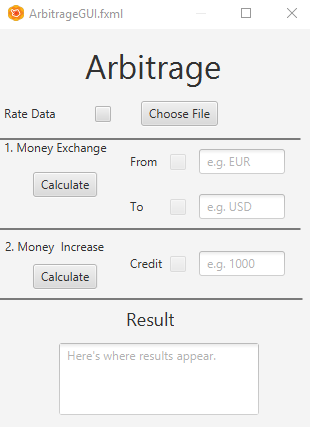
\includegraphics[scale=1]{ArbitrageGUI}
\end{center}

\begin{itemize}
\item \textbf{Podanie pliku z kursami walut:}
\begin{enumerate}
\item Naciśnij przycisk \textit{Choose file} - pojawi się okno wyboru pliku z twojego systemu.
\item Wybierz plik i zatwierdź - powrócisz do ekranu początkowego.
\item W kwadracie obok przycisku \textit{Choose file} pojawi się znaczek, potwierdzający dokonanie operacji wyboru pliku.


\includegraphics[width=5cm]{FileChosen}
\end{enumerate}
Przykładowy plik wejściowy:

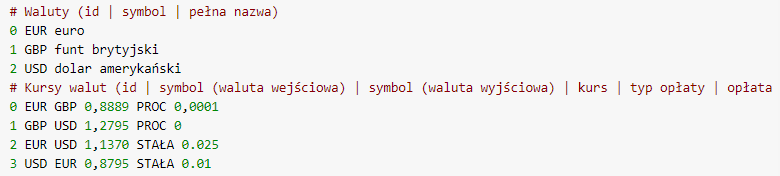
\includegraphics[width= 16cm]{FileFormat}

\item  \textbf{Korzystna wymiana waluty:}
\begin{enumerate}
\item W pierwszej sekcji (\textit{Money Exchange}) w pole tekstowe na prawo od napisu \textit{From} należy podać skróconą nazwę waluty, za którą chcemy dokonać zakupu.
\\ Po tej operacji w kwadracie po lewej stronie pola tekstowego pojawi się znaczek potwierdzający podanie skróconej nazwy waluty.
\item Poniżej, w pole tekstowe na prawo od napisu \textit{To} należy wpisać skróconą nazwę waluty, której zakupu chcemy dokonać.
\\ Po tej operacji w kwadracie po lewej stronie pola tekstowego pojawi się znaczek potwierdzający podanie skróconej nazwy waluty.
\item Następnie należy wcisnąć przycisk \textit{Calculate} znajdujący się w sekcji \textit{Money Exchange}.
\item Wynik operacji pojawi się w polu tekstowym pod napisem \textit{Result}.
\end{enumerate}
\textit{UWAGA! Należy operować na skróconych nazwach podanych w pliku z kursami walut. Wielkość liter ma znaczenie.}
\item  \textbf{Zarabianie na wymianie walut:}
\begin{enumerate}
\item W drugiej sekcji (\textit{Money Increase}) w pole tekstowe na prawo od napisu \textit{Credit} należy podać kwotę (liczbę całkowitą dodatnią), którą dysponujemy.
\item Następnie należy wcisnąć przycisk \textit{Calculate} znajdujący się w sekcji \textit{Money Increase}.
\item Wynik operacji pojawi się w polu tekstowym pod napisem \textit{Result}.
\end{enumerate}
\item\textbf{ Wyniki}
\begin{enumerate}
\item Przejścia między walutami (ścieżki) będą przedstawione w taki sposób: \emph{EUR->USD->PLN}.
\\Oznacza to, że euro wymieniliśmy na amerykańskie dolary, a dolary na złotówki.
\item W ostatniej linii wyniku wyświetlona zostanie spodziewana kwota końcowa.
\end{enumerate}
\end{itemize}

\noindent\linia
\section{Komunikaty o błędach}
W przypadku wystąpienia błędu wyskoczy okno z informacją o błędzie. 
\\\\
Przykładowe komunikaty wyglądają następująco:
\begin{itemize}
\item podano błędny plik wejściowy:

\textit{Incorrect file. Line 24 is wrong. Compare it with the file pattern.}
\item nie podano pliku, a naciśnięto przycisk \textit{Calculate}:

\textit{There was no file given.}
\item nie wypełniono wszystkich potrzebnych pól, a nacisnięto przycisk \textit{Calculate}:

\textit{Fill the missing information.}
\item podano nieprawidłową wartość w polu \textit{To} lub \textit{From}:

\textit{There is no such currency.}
\item podano w polu \textit{Credit} wartość, która nie jest liczbą całkowitą dodatnią:

\textit{The given value is not a positive integer.}
\end{itemize}
Pola tekstowe \textit{To}, \textit{From} oraz \textit{Credit} będą prawdopodobnie przystosowane do wpisywania tylko pożądanych wartości. Wtedy komunikaty o błędnym wypełnieniu tych pól nie będą się pojawiać.

\noindent\linia
\section{Testy akceptacyjne}
Testy zostaną przeprowadzone manualnie.
\\\\
Prawidłowy plik:
\\
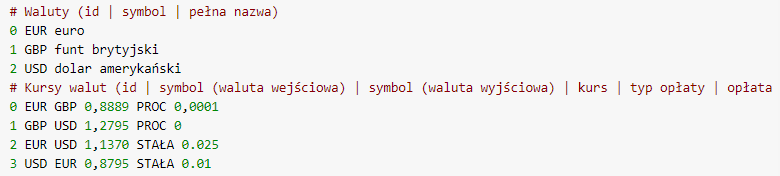
\includegraphics[width= 16cm]{FileFormat}
\\\\
Nieprawidłowy plik:
\\
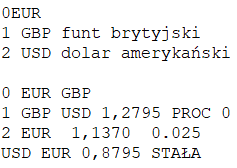
\includegraphics[width= 5cm]{FaultyFileFormat}

\begin{enumerate}
\item Należy wprowadzić nieprawidłowy plik i wypełnić pole \textit{To} wartością \textit{GBP}, a \textit{From} wartością \textit{USD}. Następnie należy wcisnąć \textit{Calculate} z sekcji \textit{Money Exchange}. Powinno pojawić się okno z komunikatem o błędzie w pliku.
\item Należy wprowadzić nieprawidłowy plik i wypełnić pole \textit{Credit} wartością 1000, a następnie wcisnąć \textit{Calculate} z sekcji \textit{Money Increase}. Powinno pojawić się okno z komunikatem o błędzie w pliku.
\item Należy wprowadzić prawidłowy plik i wypełnić pole \textit{Credit} wartością 1000, a następnie wcisnąć \textit{Calculate} z sekcji \textit{Money Increase}. W polu \textit{Results} powinna pojawić się polecana ścieżka wymiany i przewidywana kwota końcowa:
\\EUR->GBP->USD->EUR
\\1000,297170225
\item Należy wprowadzić prawidłowy plik i wypełnić pole \textit{To} wartością \textit{EUR}, a \textit{From} wartością \textit{USD}. Następnie należy wcisnąć\textit{Calculate} z sekcji \textit{Money Exchange}. W polu \textit{Results} powinna pojawić się polecana ścieżka wymiany:
\\EUR->GBP->USD
\item Należy podać prawidłowy plik i wypełnić pola \textit{To} i \textit{From} wartościami \textit{PLN} i \textit{LSD}, a następnie wcisnąć \textit{Calculate} z sekcji \textit{Money Exchange}. Powinno pojawić się okno z informacją o nieprawidłowym wypełnieniu pól \textit{To} i \textit{From}.
\end{enumerate}
\noindent\linia

\end{document}



